\chapter{はじめに}
\thispagestyle{myheadings}

% **DIOCOMO2019 ========================================================**
\section{研究背景}
コロナ禍の影響からNetflixやYouTubeやニコニコ動画といった動画共有サイトの広がりにより,映像コンテンツに触れる機会が増え,家で楽しむコンテンツの普及が進み,コンテンツをさらに気軽に楽しめるようになってきた.動画共有サイトなどに投稿された映像コンテンツは,スマートフォンなどで視聴しても楽しむことができるが,視聴コンテンツをさらに楽しめるようにしたいという視聴者のニーズも存在している。例えば,プロジェクターを使用した大画面のディスプレイでの視聴や性能の良いスピーカーを用いるなど,視聴環境をより良いものとし,コンテンツの楽しさを高めることが可能である.しかし,コンテンツが本来持っている性能を引き出すための方法であり,元からコンテンツに含まれていない3D映像や4DXなどの映像体験で新たに演出を加えるのは不可能である.
コンテンツが持っていない性能を引き出して面白さを増幅するコンテンツとして,ニコニコ動画が代表的である.その例として以下の図1.1に示す.
\begin{figure}[H]
    \centering
    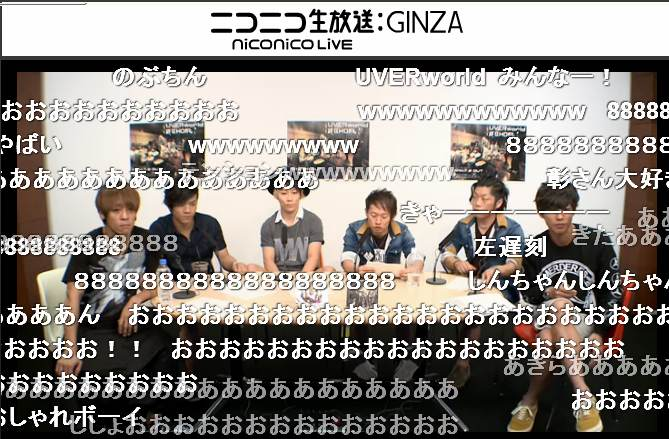
\includegraphics[width=10cm]{images/chapter1/nikoniko.jpeg}
    \caption{ニコニコ配信画面}
    \label{abst}
\end{figure}
ニコニコ動画では動画を視聴している際に視聴者が動画の任意の再生時間に対してコメントを投稿ができる.また,コメントは他のユーザからも見ることができ,文字のスタイルや大きさ,色を調整でき,動画へのリアルタイム共有が実現可能である.絵文字や記号や文字を組み合わせた視覚的表現をアスキーアートと呼ぶ.ニコニコ動画のコメントでもアスキーアートができる.コメントの投稿による感情の共有や,アスキーアートを用いた動画への表示は,コンテンツ自体にない楽しさを引き出す面白い手法である.しかし,ニコニコ動画のコメントは動画自体に重量されるものであり,動画コンテンツを視聴する際に邪魔になる.
人間の視野には中心視野と周辺視野と呼ばれる部分が存在する.中心視は視線を合わせた物をはっきりと認識する能力,周辺視は物をぼんやりとしか知覚できない代わりに全体像を瞬間的に知覚する能力である.ここで,周辺視は中心と比べて,一度に得られる情報が多く,目に入った情報の処理も無意識的に行われるので目の疲労度も少ないなどの利点がある.また,ホラー映画などのコンテンツは周辺視を利用してより視聴者の恐怖を高めるなどの手法をとっている.周辺視を効果的に使うことで動画の面白さを増幅できると考えられる.



% **DIOCOMO2020 (ryoga)====================================================**
\section{目的とアプローチ}
自宅でも映画館のような臨場感のあるコンテンツを体験可能になることが目的である。気軽に自宅でコンテンツを視聴できるようになってきている現在、ただ視聴するのみで迫力などに欠ける。コロナ禍において自宅で過ごす時間が増え、たくさんのコンテンツを視聴するようになった。そのコンテンツに対してさらなる楽しみ方を提供できるのではと考えたためである。

アプローチとして本研究ではコンテンツを視聴しているときの生体データを取得し、生体データを基にコンテンツに重畳する。コンテンツを視聴している時の生体データを取得することで感情を抜き出し、そのコンテンツにおいて盛り上がりの部分を推定する。その盛り上がりの部分が抜き出せた情報を使いコンテンツに重畳する。コンテンツへはエフェクトを画面に重畳したり、水が飛び出る、振動するなどさまざまな手法が考えられる。

\label{sec:example}


\section{論文構成}
本稿の構成は以下の通りである.2章では本研究に関連する研究として生体データする研究,重畳提示に関する研究を紹介し、3章ではコンテンツ視聴時に生体データを取得しコンテンツへ重畳提示手法についての提案を行う。第4章では評価実験を行い、本システムが生体データと重畳提示の二つについて評価する。5章ではまとめと今後の課題を述べる

